%%%%%%%%%%%%%%%%%%%%%%%%%%%%%%%%%%%%%%%%%%%%%%%%%%%%%%%%%%%%%%%%%%%%%%%%%%%

\documentclass{standalone}

\usepackage{amsmath}
\usepackage{mathptmx}
\usepackage{pgfplots}
\usetikzlibrary{external}
\tikzexternalize{e-1200-growth-factor}
\pgfplotsset{compat=1.16}

%% IEEE uses Times Roman font, so we'll default to Times.
%% These three commands make up the entire times.sty package.
\renewcommand{\rmdefault}{ptm}
\renewcommand{\ttdefault}{pcr}
\normalfont\selectfont

\begin{document}

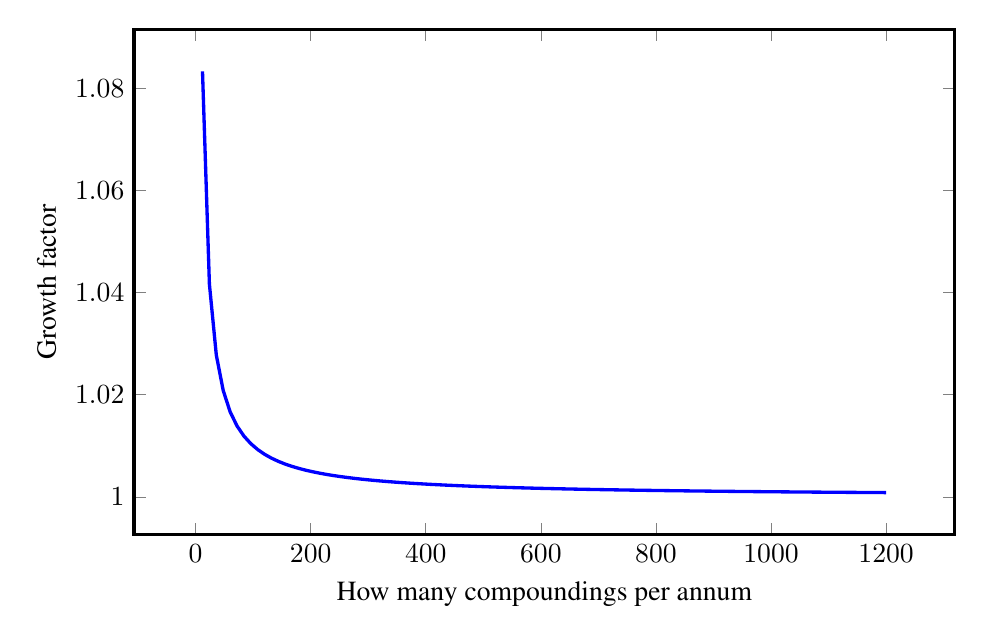
\begin{tikzpicture}
\tikzset{%%
  every mark/.append style={scale=1.0},%%
  scale=1.0%%
}
\pgfplotsset{%%
  every axis/.append style={font=\normalsize}%%
}
%%
\begin{axis}[%%
  axis line style=very thick,%%
  dotStyle/.style={very thick,blue,mark=none},%%
  enlargelimits=true,%%
  height=8cm,%%
  width=12cm,%%
  %% x axis
  xlabel={\normalsize How many compoundings per annum},%%
  xtick={0,200,400,600,800,1000,1200},%%
  xticklabels={$0$,$200$,$400$,$600$,$800$,$1000$,$1200$},%%
  %% y axis
  ylabel={\normalsize Growth factor}%%
]
%%
%%
\addplot[dotStyle] coordinates {
  (12, 1.08333333333333)
  (24, 1.04166666666667)
  (36, 1.02777777777778)
  (48, 1.02083333333333)
  (60, 1.01666666666667)
  (72, 1.01388888888889)
  (84, 1.01190476190476)
  (96, 1.01041666666667)
  (108, 1.00925925925926)
  (120, 1.00833333333333)
  (132, 1.00757575757576)
  (144, 1.00694444444444)
  (156, 1.00641025641026)
  (168, 1.00595238095238)
  (180, 1.00555555555556)
  (192, 1.00520833333333)
  (204, 1.00490196078431)
  (216, 1.00462962962963)
  (228, 1.00438596491228)
  (240, 1.00416666666667)
  (252, 1.00396825396825)
  (264, 1.00378787878788)
  (276, 1.0036231884058)
  (288, 1.00347222222222)
  (300, 1.00333333333333)
  (312, 1.00320512820513)
  (324, 1.00308641975309)
  (336, 1.00297619047619)
  (348, 1.00287356321839)
  (360, 1.00277777777778)
  (372, 1.00268817204301)
  (384, 1.00260416666667)
  (396, 1.00252525252525)
  (408, 1.00245098039216)
  (420, 1.00238095238095)
  (432, 1.00231481481481)
  (444, 1.00225225225225)
  (456, 1.00219298245614)
  (468, 1.00213675213675)
  (480, 1.00208333333333)
  (492, 1.0020325203252)
  (504, 1.00198412698413)
  (516, 1.00193798449612)
  (528, 1.00189393939394)
  (540, 1.00185185185185)
  (552, 1.0018115942029)
  (564, 1.00177304964539)
  (576, 1.00173611111111)
  (588, 1.00170068027211)
  (600, 1.00166666666667)
  (612, 1.0016339869281)
  (624, 1.00160256410256)
  (636, 1.00157232704403)
  (648, 1.00154320987654)
  (660, 1.00151515151515)
  (672, 1.0014880952381)
  (684, 1.00146198830409)
  (696, 1.0014367816092)
  (708, 1.00141242937853)
  (720, 1.00138888888889)
  (732, 1.00136612021858)
  (744, 1.00134408602151)
  (756, 1.00132275132275)
  (768, 1.00130208333333)
  (780, 1.00128205128205)
  (792, 1.00126262626263)
  (804, 1.00124378109453)
  (816, 1.00122549019608)
  (828, 1.0012077294686)
  (840, 1.00119047619048)
  (852, 1.00117370892019)
  (864, 1.00115740740741)
  (876, 1.00114155251142)
  (888, 1.00112612612613)
  (900, 1.00111111111111)
  (912, 1.00109649122807)
  (924, 1.00108225108225)
  (936, 1.00106837606838)
  (948, 1.00105485232068)
  (960, 1.00104166666667)
  (972, 1.00102880658436)
  (984, 1.0010162601626)
  (996, 1.00100401606426)
  (1008, 1.00099206349206)
  (1020, 1.00098039215686)
  (1032, 1.00096899224806)
  (1044, 1.00095785440613)
  (1056, 1.00094696969697)
  (1068, 1.00093632958802)
  (1080, 1.00092592592593)
  (1092, 1.00091575091575)
  (1104, 1.00090579710145)
  (1116, 1.00089605734767)
  (1128, 1.0008865248227)
  (1140, 1.00087719298246)
  (1152, 1.00086805555556)
  (1164, 1.00085910652921)
  (1176, 1.00085034013605)
  (1188, 1.00084175084175)
  (1200, 1.00083333333333)
};
\end{axis}
\end{tikzpicture}

\end{document}
